\section{Elementi di scienza dei dati}

\subsection{Analisi descrittiva}
Grafici e numeri vengono usati per riassumere e processare i dati trasformando l'informazione.

\begin{itemize}
    \item Si hanno troppi dati ed è difficile trarre conclusioni
    \item riassumere i dati senza perdere informazioni
    \item riassumere dipende dal task
    \item la visualizzazione dei dati è una delle parti più importanti dell'anailisi descrittiva
\end{itemize}

\subsubsection{Classificazione delle variabili}
\begin{itemize}
    \item Categoriche: (male, bene, buono, ottimo)
    \item Numeriche
    \begin{itemize}
        \item discrete
        \item continue(misurzioni del mondo reale)
    \end{itemize}
\end{itemize}

\subsubsection{Livelli di misurazione}
Per estrarre conoscenza dai dati categorici, bisogna associare loro un valore.
Un'altra Classificazione dei dati è:
\begin{itemize}
    \item Dati qualitativi: non c'è una misura fra la differenza di due dati(maschio femmina)
    \item dati quantitativi: la differenza fra due dati ha un senso(3 banane)
\end{itemize}

\begin{figure}[H]
    \centering
    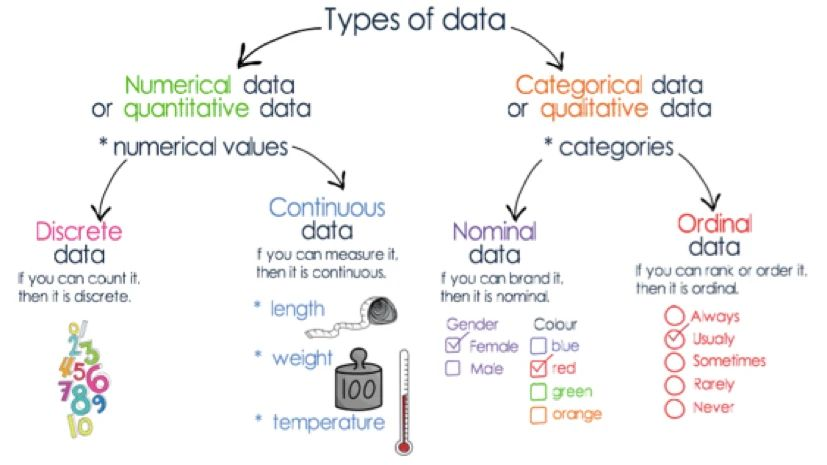
\includegraphics[width=0.7\linewidth]{imgs/1 - dati}
    \caption{Tipi di dati}
    \label{fig:tipi_di_dati}
\end{figure}

\subsection{Descrizione numerica dei dati}
\subsubsection{Misura della tendenza centrale}
I dati tendono ad un valore e usiamo:
\begin{itemize}
    \item media aritmetica
    \item mediana
    \item moda
\end{itemize}

\subsubsection{Media}
\begin{equation}
    M_a = \frac{1}{n}\sum_{i=1}^{n}x_i
    \label{eq:media}
\end{equation}
\subsubsection{Mediana}
Se i numeri presi in considerazione sono dispari, una volta ordinati, si prende quello centrale.
Se i numeri sono dispari, dopo l'ordinamento, si prende il numero successivo a quello che sarebbe il centrale.

\subsubsection{Moda}
La moda è l'elemento più frequente.

\subsubsection{Misura di dispersione: Varianza}
Qaunto i dati si discostano dalla media.
\begin{equation}
    \sigma_X^2 = \frac{\sum_{i}(x_i - \mu_X)^2}{n}
    \label{eq:varianza}
\end{equation}

\subsubsection{Misura di dispersione: Deviazione standard}
Togliendo la radice quadrata:
\begin{equation}
    \label{eq:deviazione_standard}
    \sigma = \sqrt[2]{\frac{\sum_{i=1}^{N}(X_i - \mu)^"}{N}}
\end{equation}

\subsubsection{Relazione fra due variabili: covarianza}
\begin{equation}
    cov(X,Y) = \frac{\sum{(X_i -
    \overline{X})(Y_j
    - \overline{Y})}}
    {n}
    \label{eq:covarianza}
\end{equation}

\subsubsection{Relazione fra due variabili: correlzione di pearson}
\begin{equation}
    \rho_{X,Y} = \frac{cov(X,Y)}{\sigma_X\sigma_Y}
    \label{eq:pearson}
\end{equation}



























